\documentclass[journal]{IEEEtran}
\usepackage{cite}

\usepackage{hyperref}
\usepackage[pdftex]{graphicx}
\usepackage{subfigure}
\usepackage{mathrsfs,amsmath,amsfonts}   %The amsmath package is included for \xrightarrow
\usepackage{listings}

\hypersetup{
	colorlinks=false,
	pdfborder={0 0 0},
}

\lstset{ %
  %backgroundcolor=\color{white},   % choose the background color; you must add \usepackage{color} or \usepackage{xcolor}
  basicstyle=\footnotesize,        % the size of the fonts that are used for the code
  breakatwhitespace=false,         % sets if automatic breaks should only happen at whitespace
  breaklines=true,                 % sets automatic line breaking
  captionpos=b,                    % sets the caption-position to bottom
  %commentstyle=\color{mygreen},    % comment style
  deletekeywords={...},            % if you want to delete keywords from the given language
  escapeinside={\%*}{*)},          % if you want to add LaTeX within your code
  extendedchars=true,              % lets you use non-ASCII characters; for 8-bits encodings only, does not work with UTF-8
  frame=single,                    % adds a frame around the code
  keepspaces=true,                 % keeps spaces in text, useful for keeping indentation of code (possibly needs columns=flexible)
  %keywordstyle=\color{black},       % keyword style
  language=C,                 % the language of the code
  morekeywords={*,...},            % if you want to add more keywords to the set
  numbers=none,                    % where to put the line-numbers; possible values are (none, left, right)
  numbersep=5pt,                   % how far the line-numbers are from the code
  %numberstyle=\tiny\color{black}, % the style that is used for the line-numbers
  %rulecolor=\color{black},         % if not set, the frame-color may be changed on line-breaks within not-black text (e.g. comments (green here))
  showspaces=false,                % show spaces everywhere adding particular underscores; it overrides 'showstringspaces'
  showstringspaces=false,          % underline spaces within strings only
  showtabs=false,                  % show tabs within strings adding particular underscores
  %stepnumber=1,                    % the step between two line-numbers. If it's 1, each line will be numbered
  %stringstyle=\color{black},     % string literal style
  tabsize=4,                       % sets default tabsize to 2 spaces
  title=\lstname                   % show the filename of files included with \lstinputlisting; also try caption instead of title
}


\begin{document}
\title{Tumour Classification By Volumetric Image Analysis}
\author{
	\IEEEauthorblockN{Ashley J. Robinson\\}
	\IEEEauthorblockA{	University of Southampton\\
	\href{mailto:ajr2g10@ecs.soton.ac.uk}{ajr2g10@ecs.soton.ac.uk}
	}	
}


% The paper headers
\markboth{COMP6033: Independent Research Review. $08$/$05$/$14$.}%	DRAFT REPORT.}%
{Robinson: Effective Tumour Classification Exploiting Volumetric Image Analysis}

\maketitle


\begin{abstract}

This research review covers techniques available for the classification of tumours in the human body considering practical implications of individual methods.   
An architecture is proposed to classify medical images that follows basic image processing conventions with an additional sub-module that provides non-technical confidence informations for a domain expert.  
All image processing stages are considered only for the case of volumetric images.
Using a third dimension scales up complexity because of the amount of data available but has the potential to yield better results than a 2D approach.
A combination of image processing and machine learning techniques are reviewed and a selection is made on how to populate the architecture.
These include volumetric image extraction, feature selection and classifier. 
Human supervised deployment is considered whether stand-alone or as an extension to existing medical review software.

\end{abstract}







%\begin{IEEEkeywords}
%Tumour, Classification
%\end{IEEEkeywords}



\IEEEpeerreviewmaketitle







\section{Introduction}
\IEEEPARstart{T}{his} research review covers the use of volumetric image analysis in medicine to accurately classify tumours. 
The problem is to be approached by considering only the general case where no specific area of the human body is considered.
Rather than trying to classify lung or brain tumours individually the goal is to consider what tumours have in common and given an entire image of a human body is it possible to classify tumours in any given section?
The motivation behind this is to make the most of medical scanning.
Dosages of radiation, cost and simply the time required are all reasons to reduce the number of required scans.
Making the most of any data gathered is a constructive method of scan frequency reduction.
The objective is to provide a recommendation for a system to be implemented such that a medical practitioner could use it as a tool for diagnosis.  

The architecture in Fig.~\ref{fig:Proposed} is the framework of the system to be recommended; inspired by those discussed in~\cite{ahmed2011efficacy,kumar2011classification,hau07feat,sachdeva2011multiclass,kostis03three}.
A chain of stages leads from raw data gathered from the patient to a diagnosis from a classification algorithm.
A confidence sub-block enables the domain expert to view the performance of the entire system without knowing the intricacies of operation; this requires processing to be explained with respect to their domain.
In machine learning for medical applications a classification threshold has to be selected carefully as false negatives are more serious the false positive.

Raw data is captured from the patient and passed to system for pre-processing then feature extraction.
Input patterns are produced dependent on a pre-determined list of known useful features. 
Feature reduction and normalisation is then used to frame the data as such to make the most of the classification algorithm.

\begin{figure}[!htb]
   \centering
   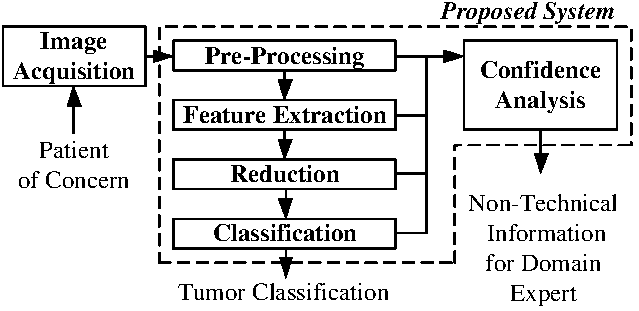
\includegraphics[width = 0.4\textwidth]{Figures/Proposed.pdf}
   \caption{Proposed system architecture.}
   \label{fig:Proposed}
\end{figure}











\section{Image Acquisition}
\label{sec:image}

A standard X-ray medical scan is tuned to produce and image of human bone.
The rays are attenuated by different materials in the body, more so by dense regions of bone, and the image is gained from this attenuation effect~\cite{kayvan2006biomedical}..  
This uses a single source and substrate to capture the image.
Taking multiple images from many different angles gathers more information and a 3D image can be made by stitching these together.
Fig.~\ref{fig:ct} describes the physical process of gathering data to be used in Computed Tomography (CT).
A ring allows images to be capture from 360$^{\circ}$ in a single plane then by moving in the orthogonal plane, in Fig.~\ref{fig:ct} through the paper, a full volumetric image of the patient can be made. 

\begin{figure}[!htb]
   \centering
   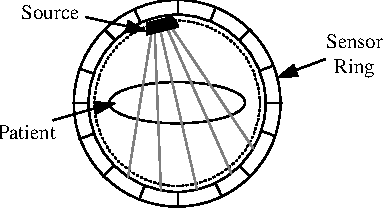
\includegraphics[width = 0.3\textwidth]{Figures/CT.pdf}
   \caption{Acquiring data from Computed Tomography. Adapted from~\cite{kayvan2006biomedical}.}
   \label{fig:ct}
\end{figure}

Any method of non-invasive image capturing in 2D can therefore be expanded to work in 3D by using the CT principle.
Different methods have trade-offs such as radiation dosages and resolution.
Ultrasound is a method of image acquisition with the advantage of a small processing overhead allowing internal organs to be viewed in real-time which is beneficial because it allows practitioners to view internal physical movement. 
It can be used for CT but higher resolution methods are usually favoured such as X-ray and Magnetic Resonance Imaging (MRI).

There are also other non-intrusive methods that do not use electromagnetic or ultrasonic waves.
Hand palpitation is a common technique used by medical practitioners to gain an impression of abnormalities near the surface of the human body. 
Electromechanical apparatus employing the same technique can be used transfer the geometry of a growth to a volumetric image~\cite{liu09haptic,wellman1997modeling}.  
Only part of the area under inspection is visible so the technique has obvious drawbacks.

Data is typically stored as a series of greyscale 2D images which are slices of the scan.
The image viewer will build 3D images as and when required using these slices.
The common medical standard for these images is DICOM which holds the slices, relative position and also patient information~\cite{dicom11nema}.
Viewing the data naturally proves problematic because it is 3D data shown in an isometric fashion on a 2D screen.
Viewing software provides interactive images as shown in Fig.~\ref{fig:3d} which allows the user to move three slices to gain an impression of the region.

\begin{figure}[!htb]
   \centering
   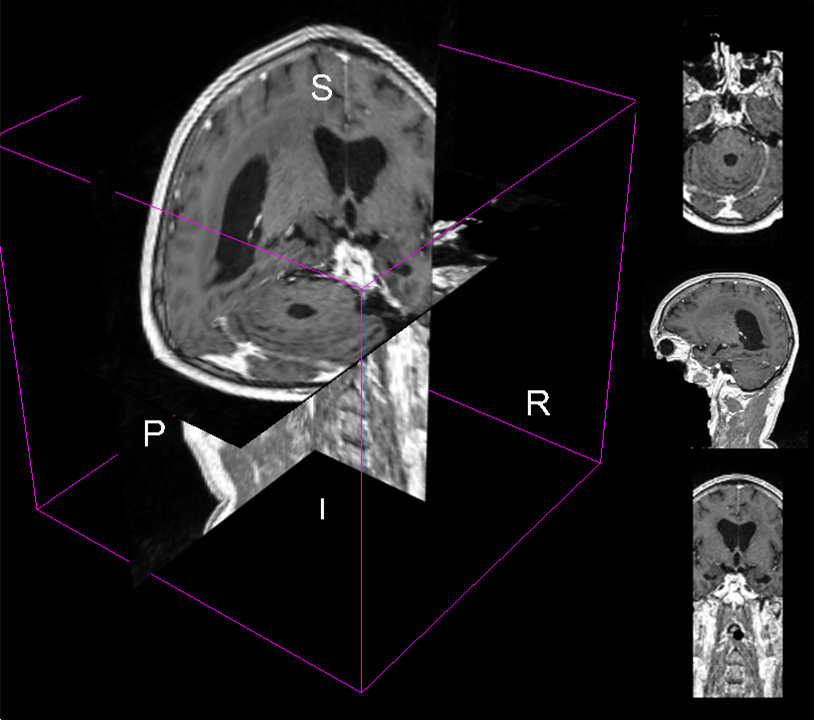
\includegraphics[width = 0.3\textwidth]{Figures/3Dview.png}
   \caption{An MRI scan of a healthy brain taken from~\cite{cia} and rendered by~\cite{slicer}.}
   \label{fig:3d}
\end{figure}












\section{Tumor Features}
\label{sec:tumor}

There are hundreds of types of tumours that can occur in the human body but they are all caused by abnormalities in cell growth~\cite{cooper1992cancer}.
Tumours are dense areas of cells in the human body and can be either benign or malignant.
Malignant tumours are considered cancers because they invade nearby normal tissue and spread therefore making them an area of concern; these are broken down in to three categories.
\emph{Carcinomas} where cells line the body and internal organs account for $90$\% of human caners.
\emph{Leukemias} and \emph{Lymphomas} which occur in the blood and lymph systems account for $8$\%.
\emph{Sarcomas} are solid regions of connective tissue which are rare.


Whether the tumor lines the host or grows independently the key to feature extraction is to differentiate normal and abnormal cell density. 
Figure~\ref{fig:ex} contains examples of identified tumors in different organs.
The brain (\ref{fig:exBrain}) and lung (\ref{fig:exLiver}) images are far simpler than the liver image (\ref{fig:exLiver}).
An image of a liver will contain other organs so these must be considered when trying to extract features.

\begin{figure}
	\centering
	\subfigure[Brain~\cite{islam12seg}]{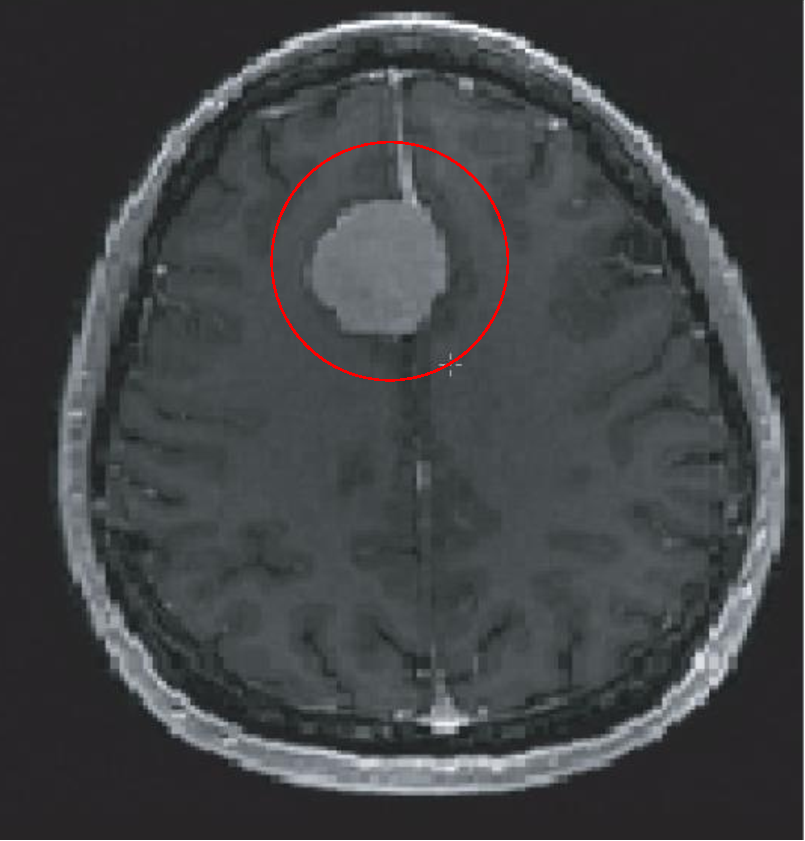
\includegraphics[width=0.12\textwidth,height=0.12\textwidth]{Figures/Brain.pdf}
	\label{fig:exBrain}}
	\subfigure[Lung~\cite{amutha13lung}]{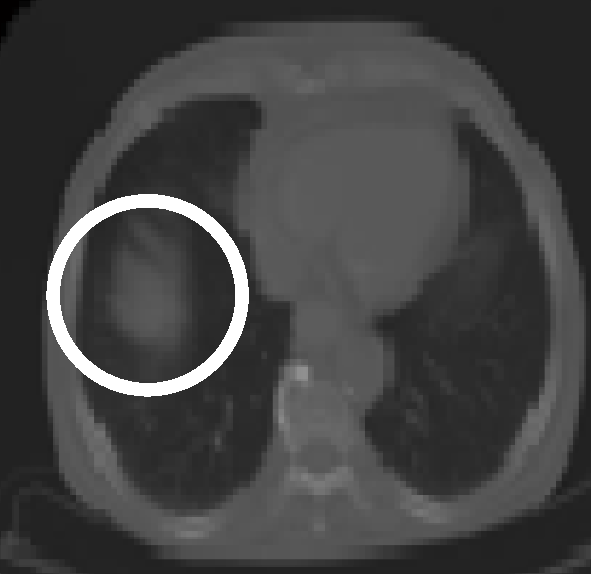
\includegraphics[width=0.12\textwidth,height=0.12\textwidth]{Figures/Lungs.pdf}
	\label{fig:exLung}}
	\subfigure[Liver~\cite{chen07mr}]{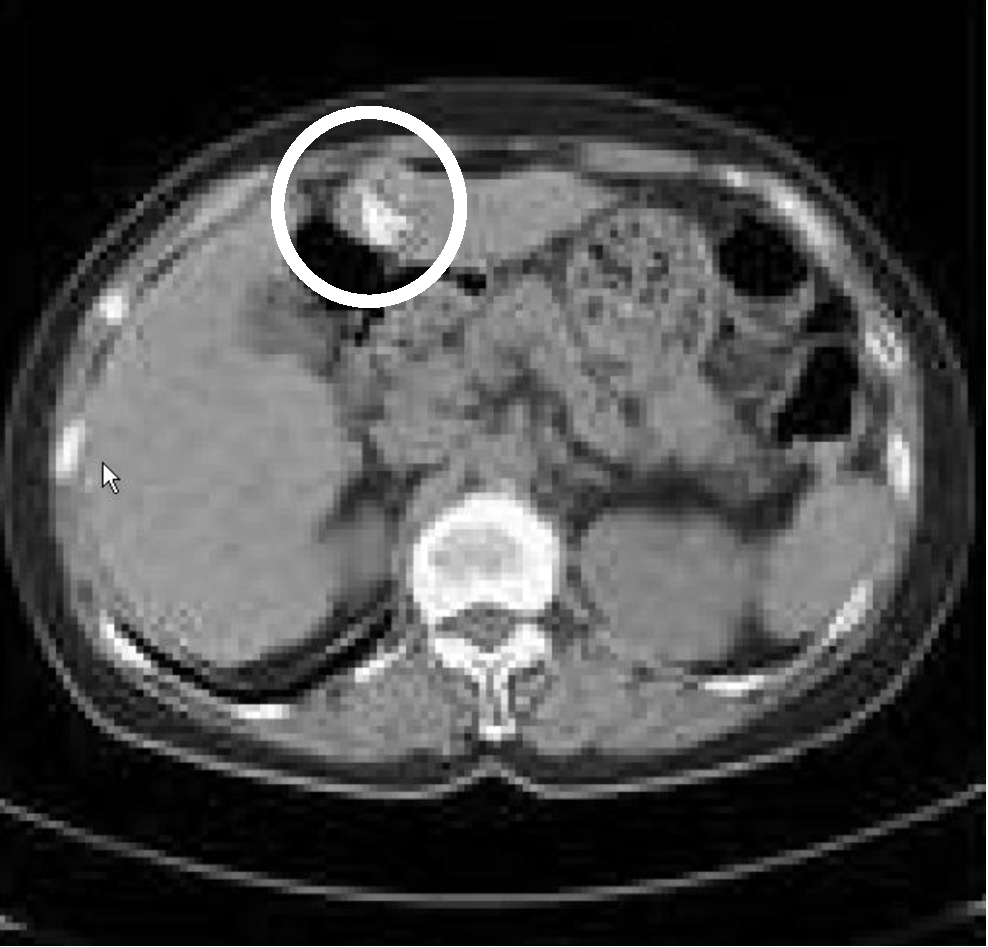
\includegraphics[width=0.12\textwidth,height=0.12\textwidth]{Figures/Liver.pdf}
	\label{fig:exLiver}}
\caption{Example MRI images containing tumors.}
\label{fig:ex}
\end{figure}











\section{Pre-processing}
\label{sec:pre}

The analogue of a pixel (picture element) in 2D images is called a voxel (volumetric element) in a 3D images.
This is exactly the same idea but with a extra dimension to form a cube~\cite{lohmann1998volumetric}.
They can be considered cubes but also points which may make visualisation and processing easier to understand.
Fig.~\ref{fig:neighbourhood} describes how voxels are packed and three different neighbourhoods the can be considered when inspecting one voxel. 
Considering voxels to have larger neighbourhoods can increase the time complexity of some algorithms.


\begin{figure}
	\centering
	\subfigure[6]{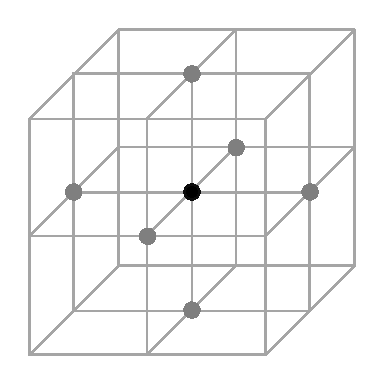
\includegraphics[width = 0.12\textwidth]{Figures/6N.pdf}
	\label{fig:neighbourhood6}}
	\subfigure[18]{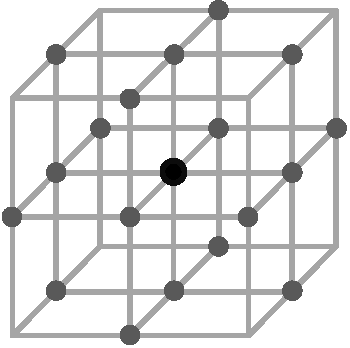
\includegraphics[width = 0.12\textwidth]{Figures/18N.pdf}
	\label{fig:neighbourhood18}}
	\subfigure[26]{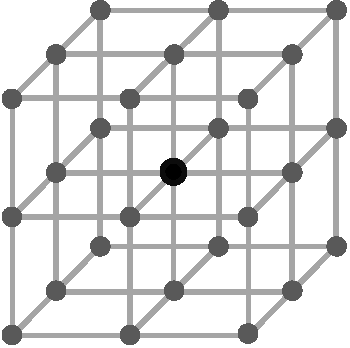
\includegraphics[width = 0.12\textwidth]{Figures/26N.pdf}
	\label{fig:neighbourhood26}}
\caption{Voxel Neighbourhoods~\cite{lohmann1998volumetric}.}
\label{fig:neighbourhood}
\end{figure}


The provided raw data needs to be converted from the delivery format of the acquisition technology to a raw 3D matrix ready for generic processing.
Watermarking, which may have been inserted for human review, should also be removed at this stage. 
This is trivial in theory but requires a database of artefacts or manual review to accomplish.
There are also techniques, not considered in this paper, which can be applied just to the slices of a volumetric image which may be used to reduce processing overheads~\cite{harauz86exact}.

There are different techniques available to enhance the image captured or ensure it is correctly formatted for further processing.
This is considered as a mapping from an original image to a new image, $\textbf{I} \mapsto \textbf{I}'$, using only information from the original image.

\subsection{Histogram Operations}

An image histogram is a mapping from an image to a 2D plot of the frequency of voxel intensity; possible since voxels can have a discrete value of intensity within a fixed range.
This contains information on the type of material seen in the image, if it can be determined from intensity, and how much of that material is used to form the entire image.
Image enhancement can be performed using point operations with information from the histogram.
This is a very fast methods of image enhancement as it is direct voxel-to-voxel mapping; see Eq.~\eqref{eqn:point}. 
Normalisation stretches the histogram to cover all available values of intensity therefore improving contrast.
Equalisation attempts to flatten the histogram by distributing intensity~\cite{nixon02feature}.


\begin{equation}
	I'(u,v,w) = \alpha(u,v,w)I(u,v,w)
	\label{eqn:point} 
\end{equation}



\subsection{Spatial Filtering}
Spatial filters use the neighbourhood of voxels to create a new value for each voxel in an image. 
The original image is mapped to a new image through a filter kernel, as described in Eq.~\eqref{eqn:kernel}.
The filter kernel is a fixed dimension sub-image with a weighting on each voxel that is applied to every voxel in the original image.
This is spatial convolution.
If the filter kernel contains all ones it is known as a \emph{box filter} and performs smoothing on the image to remove noise.
A Gaussian filter performs better by placing a higher weighting on the central voxel and less on the extreme voxels~\cite{lohmann1998volumetric}.
The edge voxels of an image do not have a complete set of neighbours therefore performing spatial filtering will reduce the total size of the image in further processing.

\begin{equation}
	I'(u,v,w) = \sum\limits_{(i,j,k) \in R_H} I(u + i,v + j, w + k)H(i,j,k)
	\label{eqn:kernel} 
\end{equation}



\subsection{Frequency Filtering}
The Fourier transform, as used spatially on 2D images, can be extended to 3D images.
A Discrete Fourier Transform (DFT) for a $N^3$ voxel image is held in Eq.~\eqref{eqn:dft}.
The spatial filtering process performs convolution so once an image is in the frequency domain the same effects can be achieved using multiplication.
It may prove more efficient to filter an image in the frequency domain rather than space if the required filter kernel is large.
Band-pass and notch filter operations can also be perform in the frequency domain.
Eq.~\eqref{eqn:same} provides the same result as Eq.~\eqref{eqn:kernel} using the transform from Eq.~\eqref{eqn:dft}.

\begin{equation}
	F_{u,v,w} = \frac{1}{N^{\frac{3}{2}}} \sum\limits_{x=-\frac{N}{2}}^{\frac{N}{2}-1}\sum\limits_{y=-\frac{N}{2}}^{\frac{N}{2}-1}\sum\limits_{z=-\frac{N}{2}}^{\frac{N}{2}-1}I_{x,y,z}e^{-j\frac{2\pi}{N}(ux + vy + wz)}
	\label{eqn:dft} 
\end{equation}

%\begin{equation}
%	\textbf{F} = \mathcal{F}(\textbf{P}),\:\:\textbf{P} = \mathcal{F}^{-1}(\textbf{F}) 
%	\label{eqn:ft} 
%\end{equation}

\begin{equation}
	\textbf{I}' = \mathcal{F}^{-1}(\mathcal{F}(\textbf{I})*\mathcal{F}(\textbf{H})) = \mathcal{F}^{-1}(\textbf{I}**\textbf{H})		% Arrow doesn't work, implied matrices?
	\label{eqn:same} 
\end{equation}


\subsection{Anisotropic Diffusion}
Anisotropic diffusion is a powerful technique used to enhance images where it is possible to remove noise yet retain edges.
The technique has been expanded from common 2D applications to 3D medical usage on MRI data~\cite{nakh11three}.
The diffusion effect has the same outcome as a low pass filter with reasonably adjusted values for $\Delta t$ and the decay constant.
The spatial scaler $\mathbf{k}$ is a function of the image and on edge must preserve edge by setting $k(x_{edge},y_{egde},z_{edge},t) = 0$.
Using Eq.~\eqref{eqn:anisotropic} an iterative approach is provided in Eq.~\eqref{eqn:anisotropic_it} where the original image it the value of $\mathbf{I}$ at time zero.
Iteration monitoring and reasonable scalar values in the function $\mathbf{k}$ are required to produce a good outcome.
Edge detection methods to be used for $\mathbf{k}$ are discussed in~\cite{nixon02feature} but for edge critical processing Canny edge detection is suitable~\cite{canny86edge}. 

\begin{equation}
	\frac{\partial \mathbf{I}}{\partial t} = \mathbf{k(\mathbf{I})} \mathbf{\nabla}^2 \mathbf{I},\:\:\mathbf{k},\mathbf{I} \in \mathbb{R}^4
	\label{eqn:anisotropic} 
\end{equation}

\begin{equation}
	\mathbf{I}_{t + \Delta t} = \mathbf{I}_t + \Delta t\mathbf{k}(\mathbf{I}_t)\mathbf{\nabla}^2\mathbf{I}_t
	\label{eqn:anisotropic_it} 
\end{equation}















\section{Feature Extraction}
\label{sec:extraction}

High level feature extraction of volumetric shapes should be used on the input image.
These high intensity regions may be organs walls or bones but should also include potential tumors.




\subsection{Active Contours}

Expanding upon common 2D implementations active contours can be used to extract shape information from volumetric images.
Eq.~\eqref{eqn:contour_v} contains the standard energy minimisation function expanded for volumetric images~\cite{nixon02feature,skalski13automatic}. 

\begin{equation}
	E = \int_0^{1} E_{int}(\mathbf{v}) + E_{ext}(\mathbf{v}) + E_{con}(\mathbf{v})\:ds,\:\:\mathbf{v}(s) \in \mathbb{R}^3
	\label{eqn:contour_v}
\end{equation}













\section{Feature Selection}
\label{sec:selection}

Commonly large datasets contain some features in the input space will be have no effect upon or even a reduce the performance of a classifier.
It is naive to use just the raw image data.
Tumor features for extraction have been considered in section~\ref{sec:tumor} which already makes better use of data. 
Mapping input data into a lower dimensional space is possible and can improve performance but if ill-applied can remove key features.
A brute-force would approach would find the optimal combination of features but the input space is expected to be too large, $2^n$, to be completely shattered within reasonable execution time. 



\subsection{Sequential Floating Search (SFS)}

This heuristic algorithm is applied to tumor classification in~\cite{hau07feat}.
It is possible to start from either the full or empty set of features then iteratively add and remove features to improve the performance of the classifier. 
A performance function is required for set comparison. 
Listing~\ref{lst:sfs} contains the algorithm starting from an initial subset of no features and repeated until convergence.

\lstinputlisting[label=lst:sfs,caption=SFS Algorithm]{Code/sfs.txt}



\subsection{Stochastic Approaches}
A Random Mutation Hill Climber (RMHC) can move in the feature selection space from an initial starting point but will never reduce in performance.  
This does not handle a landscape with many local maxima well and may not produce a reasonable solution.
Genetic algorithms are more computationally expensive as they require a population of solutions using crossover and mutation to converge on a suitable solution.   
Whether it out performs a RMHC depends on the performance landscape but using a population of solutions is certainly more thorough.    
Simulated annealing can be used to move between solution neighbours subject over a fixed number of iterations.
A cooling schedule is used to except negative moves in performance with a probability the is a function of the cooling variables. 


\subsection{Principle Component Analysis (PCA)}
PCA is a common technique used for dimensionality reduction by ranking dimensions in order of variance~\cite{pearson01pca}.
This will rank the features so that only the first $L$ are passed on for further processing. 
The other dimensions can simply be removed but if the effect of a low variance dimension is important to classification this can reduce performance.
Eq.~\eqref{eqn:PCA} shows how the original input pattern is mapped to a reduce pattern by subtracting the mean of all patterns and multiplying with the projection matrix.
The projection matrix is built by finding the covariance matrix of the input patterns then ranking the eigenvectors by the eigenvalues and deleting as required.
Performance feedback from training can be used to select appropriate $L$ value.

\begin{equation}
	\boldsymbol{z} = \boldsymbol{P}(\boldsymbol{x} - \boldsymbol{\mu})
	\label{eqn:PCA}
\end{equation}












\section{Classification}
\label{sec:class}

Classification must differentiate between extracted geometric shapes that are normal and those which may potentially be tumors.
Tumors will also be attached to normal internal body parts so the classifier must be able to handle any abnormalities in organs.
Supervised and unsupervised techniques for classification even thought labelled datasets have not yet been sourced.


\subsection{Artificial Neutral Networks (ANNs)}
ANNs contain summation nodes where data is propagated through weighted connections resulting in a final output. 
As a supervised technique parametric weights are trained by propagating the error backwards through the network.
Multilayer nets can provided non-linear separation functions and increase the number of layers only increase the possible function complexity.



\subsection{Support Vector Machines (SVMs)}
An SVM classifier builds a separation margin supported by the close data points draw a separation function from the middle of this margin.
A linear maximum-margin hyperplane is produce but non-linear data can also be separated by using the kernel trick. 
This is a mapping of the input space into a higher dimensional space so that becomes linearly separable.
The hyperplane is then mapped back to the original input space.



\subsection{Boosting}
Boosting is the practice of combining different techniques together and drawing an output based on many sub-classifier.





\section{Conclusions}
\label{sec:conclusions}

It is clear that this tool can't be used as a hard and fast method of tumour diagnosis but instead as a valuable tool for image reviewers.
Software packages designed for medical image review, such as~\cite{slicer}, have bidirectional interfaces to custom extensions.
Implementing this system as an extension would remove many overheads required in data handling but reduce the scope for optimisation.
The feedback from the entire process would be a checklist which the user must manually review and waive if incorrectly identified. 










\bibliographystyle{ieeetran}
\bibliography{references}

\end{document}


